%Master document for paper.
%Created MS 1/30

\documentclass[psfig,12pt,notitlepage]{article}
\usepackage{axodraw4j}
\usepackage[text={6.5in,9in},centering]{geometry}               % See geometry.pdf to learn the layout options. There are lots.
\geometry{letterpaper}                   % ... or a4paper or a5paper or ... 
%\geometry{landscape}                % Activate for for rotated page geometry
\usepackage[parfill]{parskip}    % Activate to begin paragraphs with an empty line rather than an indent
\usepackage{subfigure}
\usepackage{graphicx}
\usepackage{setspace}
\usepackage{color}
\usepackage{amssymb}
\usepackage{amsmath}
\usepackage{listings}
\usepackage{epstopdf}
\usepackage{epsfig}
\usepackage{psfig}

\DeclareGraphicsRule{.tif}{png}{.png}{`convert #1 `dirname #1`/`basename #1 .tif`.png}
\usepackage{cite}


\begin{document}

\title{Measurement of Weak Coupling Constant Using Mass and Lifetime of $\mu$ Leptons}
\author{Maria Baryakhtar \footnote{Produced a, b, c} \and Steven Schowalter \footnote{Produced d, e, f} \and Maximilian Swiatlowski \footnote{Produced g, h, i}}

\maketitle

\begin{abstract}
We present our measurements of the lifetime and mass of cosmic ray
muons. The detection of muons is performed at sea level using a simple
system of three scintillators and photomultiplier tubes. We find the
average lifetime of the muon to be $\tau{\mu} = 2.12 \pm .16 \mu$s,
which is in good agreement with the accepted value of $2.20 \mu$s
\cite{pdg}. The muon mass is measured to be $m_{\mu} = 120 \pm 20$
MeV/c$^2$, which includes the accepted value of $105.66$ MeV/c$^2$
\cite{pdg}. These measurements are used to calculate the Fermi
coupling constant $G_F$. Our value of $G_F$ is determined to be $3.0
\pm 1.3\times 10^{-59}$ J m$^3$, which is in correspondence with
$4.3\times 10^{-59}$ J m$^3$, the experimentally established value
\cite{pdg}. This experiment allows us to use a low energy setup to
successfully study the weak interaction.


\end{abstract}



\tableofcontents
\setcounter{tocdepth}{2}
\listoffigures


\clearpage

%Introduction body
%Created MS 1-30

\section{Introduction}\label{introduction}

The muon is a fundamental particle produced in the upper atmosphere as
a secondary product of cosmic ray collisions with atmospheric
molecules. It decays via the weak interaction into an electron and two
neutrinos, with a mean decay lifetime of $2.2~\mu$s, longer than
every known particle other than the neutron \cite{pdg}. With muons
comprising most of the cosmic ray flux at sea level, the muon is a
good candidate for the study of the weak force \cite[p.~8]{rossi}.

Our experiment consists of two main components: the muon lifetime
measurement and the muon mass measurement. In
Section~\ref{background}, \emph{Background}, we introduce the
theoretical basis for muon creation and decay as well as the
motivation for lifetime and mass measurements and $G_{F}$ calculations. We describe the
experimental setup for muon detection which consists of a system of
three scintillators and photomultiplier tubes (PMTs) in
\emph{Instrumentation} (Section~\ref{instrumentation}). Using this
system, the cosmic ray muons passing through the scintillators and
their decay products can be detected, along with the energy of these
particles (as described in Section~\ref{procedure}, \emph{Procedure}). In Section~\ref{resultsanddiscussion}, \emph{Results and Discussion}, the muon lifetime and
mass results are presented with the relevant statistical analysis of
data and compared to previous experimentally established
values. Finally, we use the muon mass and lifetime values to calculate
the Fermi coupling constant $G_F$ that describes the strength of weak
interactions.


%Background body
%Created MB 04-12

\section{Background}\label{background}

The $^4$He atom is one of the most simple and symmetric systems
among the elements, as it has a filled innermost electron shell and no
overall electric or magnetic moment or angular momentum
\cite{atkins}. Due to the symmetric nature of helium atoms, the
interaction between them is very weak and therefore $^4$He liquifies
at an extremely low temperature of $4.21$ K. A more
interesting transition occurs at $2.17$ K, at which point liquid
helium takes on several unique properties. Below this temperature,
termed the $\lambda$-point, $^4$He\footnote{Although the isotope
  $^3$He is also capable of producing these effects, the transition
  temperature is much lower, at $3\times 10^{-3}$ K, and is
  unreachable with the cryogenic technology available to us. Thus, in
  the remainder of the paper, the isotope $^4$He is implied unless
  stated otherwise.}  acquires extremely high thermal conductivity,
negligible viscosity, and the ability to propagate temperature waves
(second sound); in addition, there is a $\lambda$-shaped discontinuity
at the transition point in the heat capacity of liquid helium, which
gives the $\lambda$ point its name. To distinguish the two phases of
liquid helium, the liquid is referred to as helium I above the
$\lambda$-point and helium II below the $\lambda$-point
\cite{tilley}. The investigation of the properties of helium II
mentioned above will be the focus of this paper.

\subsection{The Two-Fluid Model}\label{thetwofluidmodel}

First proposed by Landau in 1941\cite{landau}, the two fluid model 
is a key theoretical framework for explaining the
unusual properties of He II, In this theory, the liquid below the $\lambda$-point
can be viewed as being composed of two noninteracting fluids: a
superfluid component with density $\rho_s$ and a normal component with
density $\rho_n$, such that the total density $\rho$ is given as the
sum of the two components:
\begin{equation}
\rho = \rho_s + \rho_n
\label{eqn:density}
\end{equation}

and the total current density of He II is given by
\begin{equation}
\mathbf{j} = \rho_s\mathbf{v_s} + \rho_n\mathbf{v_n}
\end{equation}

where $\mathbf{v_s}$ and $\mathbf{v_n}$ are the velocities of the
superfluid and normal fluid, respectively \cite{tilley}. Then, the
behavior of the fluid can be understood in terms of the different
characteristics of the two components: while the normal fluid acts
according to the regular laws of fluid mechanics and satisfies the
Navier-Stokes equation, the superfluid carries zero entropy and flows
with zero viscosity. Furthermore, it is important to note that the two
components are non-interacting-- \emph{i.e.}, there is no transfer of
momentum between the two fluids-- and that they are
not physically distinct and cannot be separated \cite{tilley}.

The physics of Bose-Einstein condensation allows for further
understanding of the superfluid. The idea of describing the superfluid
as a Bose-Einstein condensate was originally proposed by Tisza in 1940
and later incorporated into Landau's theory \cite{tisza}. The
superfluid can be viewed as an interacting Bose-Einstein condensate
system occupying a single macroscopic quantum state, whereas the
normal fluid consists of the excitations (phonons and rotons) of the
superfluid. As temperature decreases from $2.17$ K to $0$ K the fraction
of superfluid increases from zero at the $\lambda$-point to unity at
absolute zero, and the excitations decrease to zero, as in Fig.
\ref{fig:twofluid}\cite{andro}.

\begin{figure}[ht]
\begin{center}
\includegraphics{./figures/twofluid.eps}
\caption{\small{Relative fractions $\rho_s/\rho$ and $\rho_n/\rho$ of
    the superfluid and normal components in He II\cite{andro}. The
    superfluid effects disappear above the $\lambda$-point.}}
\label{fig:twofluid}
\end{center}
\end{figure}


\subsection{Heat Transfer and Second Sound}\label{heattransferandsecondsound}

\subsubsection{Thermal Conductivity}\label{thermalconductivity}
The thermal conductivity of He II is very high, and tends to infinity
for small heat currents \cite{tilley}, making the fluid intolerant to
temperature gradients. This property explains the visually noticeable
transition from He I to He II with decreasing temperature.  While
boiling is easy to observe in He I, as the temperature drops past the
$\lambda$-point the bubbling ceases immediately because a sufficient
temperature gradient cannot be established for a bubble to
form \cite{tilley}.


\subsubsection{Frictionless Flow}\label{frictionlessflow}
Another property of helium II is that the superfluid component is able
to flow without energy dissipation. Because a superfluid flows with
zero friction, it is possible to construct a barrier which permits
superfluids, but not normal fluids, to flow. One such barrier is
tightly pressed crushed glass, which creates winding paths on the
order of $100$ $\mu$m in diameter. Then, if a temperature gradient is
established across such a barrier, the only possible flow is from the
superfluid, and the superfluid will flow toward the higher
temperatures in order to reduce the gradient. As a qualitative
demonstration of this property, this experiment seeks to observe the
`fountain' effect, where the superfluid rushes through the barrier
with enough pressure to create a fountain on the opposite side.

\subsubsection{Second Sound}\label{secondsound}
While the superfluid fraction cannot directly transfer heat, it
is able to balance temperature gradients through an exchange of the
relative concentrations of the two components $\rho_n$ and
$\rho_s$, not through the standard methods of conduction and convection. As seen in \ref{fig:twofluid}, at lower temperatures the
fraction of superfluid increases and the fraction of normal fluid
decreases, so it is possible to think of the superfluid component as
`cold' and the normal component as `hot' \cite{atkins}. Thus, instead
of balancing temperature, it is possible to equivalently balance the
relative fraction of superfluid and normal fluid in different regions:
to accomplish this, superfluid flows up temperature gradients while
normal fluid flows toward lower temperatures.

This method of heat propagation in He II leads directly to the
definition of a different kind of wave possible in the fluid: second
sound. The term is defined in contrast to sound, known as first sound,
which is a pressure wave and travels via a variation of
density. Second sound is a temperature wave, and propagates instead
via the out-of-phase movement of superfluid and normal fluid past each
other, with constant total density at each point
\cite{atkins}. Because temperature travels as a wave in He II, it is
relatively dissipation-free, making it possible to measure the speed
of second sound propagation \cite{atkins}.

\subsection{Heat Capacity}\label{heatcapacity}

\subsubsection{Specific Heat of Metals}\label{specificheatofmetals}

According to the Debye theory of solids \cite{schroeder}, two factors
contribute to the specific heat of metals. One, due to the effect of
conduction electrons, increases linearly with temperature:
\begin{equation}
C_{v,a} = \alpha T
\end{equation}

and the other, due to phonon contributions, has a cubic relationship:
\begin{equation}
C_{v,b} = \beta T^3
\end{equation}

giving a total specific heat of:
\begin{equation}\label{formula:cuspecificheat}
C_v=  \alpha T + \beta T^3
\end{equation}

where $\alpha$ and $\beta$ are constants that depend on the material
and are generally determined experimentally. This model is especially
accurate at low temperatures, and we use the relationship in Eqn.
\ref{formula:cuspecificheat} to fit the heat capacity of the copper
cell which holds the liquid helium.

\subsubsection{Specific Heat of Liquid Helium}\label{specificheatofliquidhelium}

The temperature dependence of the heat capacity of liquid helium is
unique to this system. The transition point from helium I to helium II
is named after the heat capacity dependence: the plot of heat capacity
\emph{versus} temperature resembles the letter $\lambda$. Below $1$ K, the
heat capacity is nearly zero; as the temperature increases from $1$ K to
$2.17$ K, the heat capacity increases rapidly, with an apparent
discontinuity at the $\lambda$-point, where heat capacity seems to go
to infinity. Increasing the temperature still further, the heat
capacity drops to a minimum after the $\lambda$-point, and slowly
increases as the temperature reaches the helium boiling point
\cite{atkins}.

We measure the specific heat under saturated vapor pressure $C_{sat}$,
which is related to the specific heat at constant pressure, $C_p$, by
\begin{equation}\label{formula:satspecificheat}
C_{sat} = C_p - TV\alpha\left(\dfrac{dp}{dT}\right)_{v.p.c.} 
\end{equation}

where $\alpha$ is the coefficient of expansion and
$\left(\frac{dp}{dT}\right)_{v.p.c.}$ is the slope of the vapor
pressure curve \cite{atkins}. According to Atkins, below $2.5$ K, the
difference between $C_{sat}$ and $C_p$ is less than $1\%$, but it
increases to a significant fraction of $10\%$ at $4$
\cite{atkins}. While it is difficult to control the volume and
pressure of the helium sample in the setup, the liquid helium
remains in equilibrium with the helium vapor as temperature increases,
enabling the measurement of $C_{sat}$.

\subsection{Superfluid Density}

It is possible to derive the density fraction of the superfluid from
several other helium II properties. In particular, the relationship
between velocity of second sound, $u_2$, and the relative fractions of
the fluids was derived analytically by Landau and is given by

\begin{equation}
u_2^2 = \frac{\rho_s}{\rho_n}\frac{T S^2}{C}
\label{soundspeed}
\end{equation}

where $S$ and $C$ are the entropy and specific heat of the liquid and
can be measured experimentally \cite{atkins}. The speed of second
sound decreases with increasing temperature, going to zero at the
$\lambda$-point, where the superfluid fraction disappears. We measure
both specific heat and second sound velocity.  Therefore, using
established values for entropy \cite{brooks}, we can calculate the
fraction of superfluid and normal fluid as a function of temperature.


\section{Instrumentation}

In order to detect muon and electron events, signals from scintillators are correlated and matched against an expected pattern. The next section will discuss how these are used to generate lifetimes; here, we focus on describing the apparatus and problems associated with it.

\subsection{Scintillators}

The scintillator consists of polystyrene ($\mathrm{C}_{8}\mathrm{H}_{9}$, with density $1.08 \pm .09 \frac{\mathrm{g}}{\mathrm{cm}^{3}}$) doped with a phosphorous material, p-terphenyl. When ionizing radiation passes through the material a light pulse is emitted. The light flash is detected by the photomultiplier tubes placed at the ends of the scintillator. The photomultiplier uses a high voltage (on the order of 1000 V) to convert the light pulses into a cascade of electrons more or less linearly (i.e., the amplitude of the electrical signal from the photomultiplier is linearly correlated to the energy of the ionizing radiation). The signals from the photomultiplier is then fed into a bank of discriminators, which output a fixed width voltage pulse after detecting a voltage pulse above a given threshold. These signals are then fed into the logic which determines events.

\subsubsection{Efficiency Optimization}

Many different factors come into the consideration for choosing the settings at which the run the scintillators. The most obvious is the drive to maximize efficiency of the detectors so as to maximize muon count; this would require setting the voltages as high and the threshold levels as low. The other primary concern is noise, which increases at higher voltages and lower thresholds; this concern keeps voltages lower and thresholds higher.

The optimization technique relies on the very high number of muons that go straight through all detectors. As most muons are very high energy when they reach the surface of the earth, nearly the entire flux from the atmosphere passes through all the detectors without stopping. Thus, by taking the ratio of the number of events detected by all three detectors as compared to the number detected by just two of the detectors, we can get an approximation of the efficiency of the excluded detector. The ratio should be near 1 for something perfectly efficient, as losses from solid angles and muons which stop in the detectors are incredibly small as compared to the total muon flux.

Initial data runs were taken with higher efficiency (as high $99\%$ efficiency for the middle detector, 

%Procedure body
%Created MB 04-12

\section{Procedure}\label{procedure}



%Results and Discussion body
%Created MS 1-30

\section{Results and Discussion}

\subsection{Determination of Muon Lifetime}

By constructing the logic (system) discussed in the previous section, we can determine when a muon comes to rest in the middle scintillator and correspondingly produce a signal denoted the START signal.  Likewise, we can determine when the stopped muon decays by observing the production of an electron with downward velocity.  The signal that is produced is denoted the STOP signal.  These signals can then be passed from a scope to a LabView program via GPIB.  By observing the duration between START and STOP pulses the time we are able to measure the time it takes for a stopped muon to decay.  Essentially this time is the lifetime of an individual muon.  

By measuring and recording these durations 

\subsubsection{Error Analysis}

\subsection{Determination of Muon Mass}

\subsubsection{Error Analysis}

\subsection{Determination of Weak Force Coupling Constant}




\newpage

\appendix

\begin{center}
\begin{Large}
\bfseries{Appendices}
\end{Large}
\end{center}

%appendix blhablhaakljfdldskj
%Created MB 03-01

\section{Muon Mass Calibration}

For heavy ($\mu$ and heavier) charged particles passing through
matter, the amount of energy deposited depends on the incident
momentum of the particle. The relationship is given by the Bethe-Block
equation \cite{bichsel}:

\begin{equation}
-\frac{dE}{dx} = Kz^2\frac{Z}{A}\frac{1}{\beta^2}\left[\frac{1}{2}ln\frac{2m_ec^2\beta^2\gamma^2T_max}{I} - \beta^2 - \frac{\delta(\beta\gamma)}{2}\right]
\end{equation}

where $\beta = v/c$ and $\gamma = 1/\sqrt{1 - \frac{v_{\mu}^2}{c^2}}$
are of the incoming particle, and the other parameters are constants
or properties of the material.

The 

\begin{figure}[h]
\begin{center}
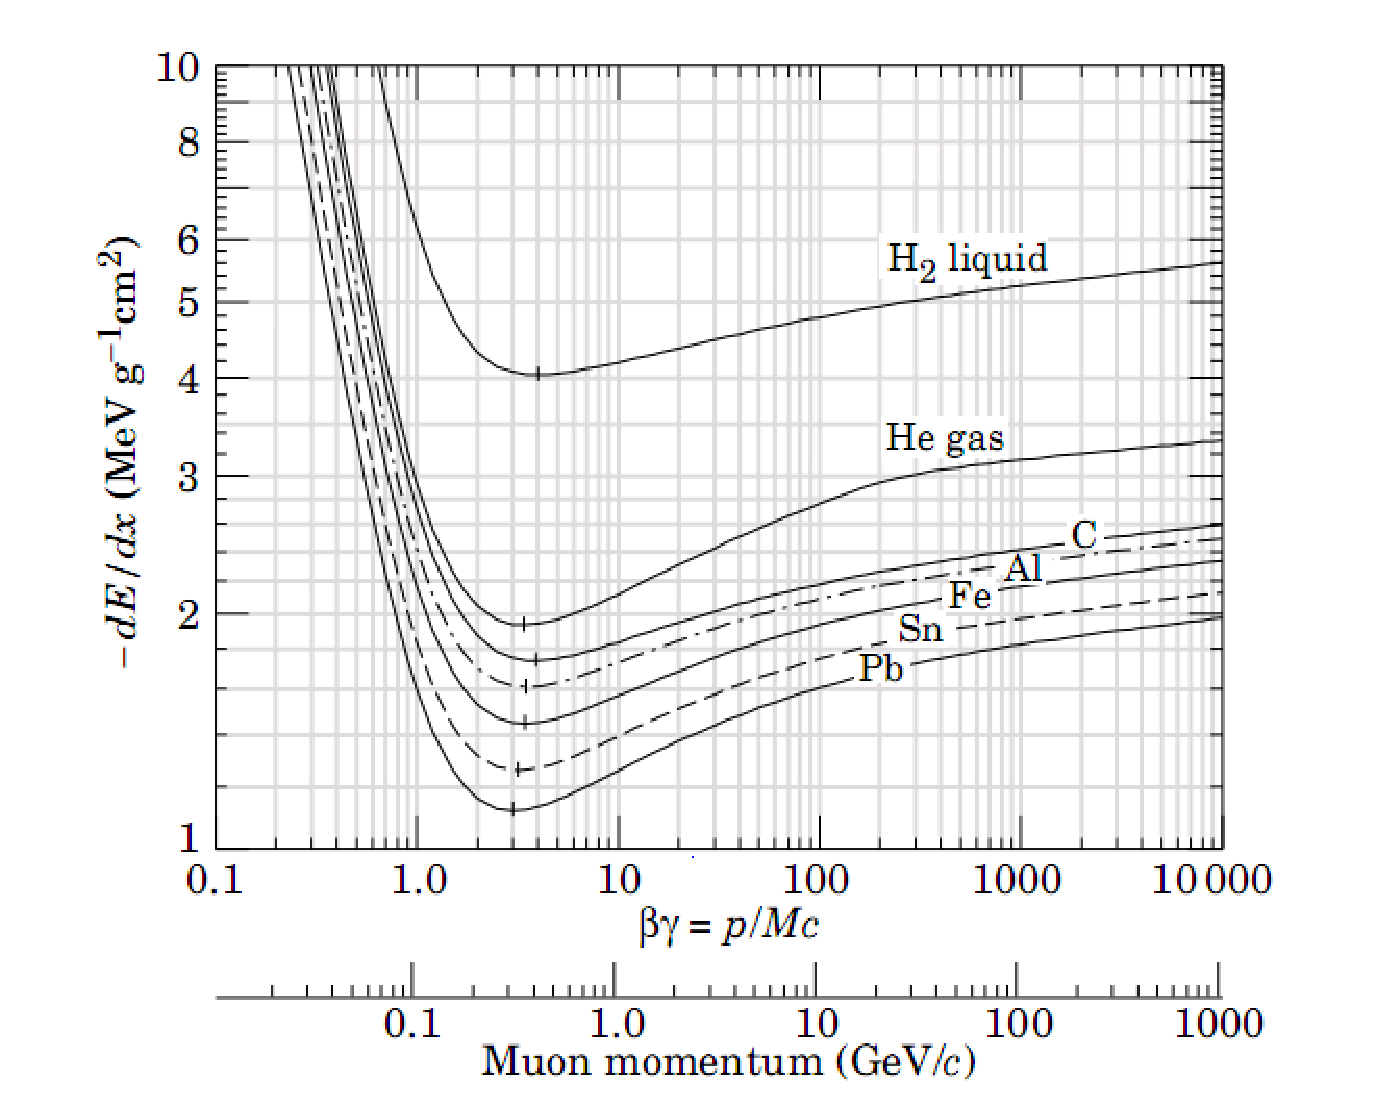
\includegraphics[width = 140mm]{figures/energy_loss.eps}
\caption{\small{Mean energy loss in various materials. In our
experiment, the scintillator consisted of carbon and hydrogen, so the
minumum ionization energy was determined by weighing the C and H
values according to mass ratio \cite{bichsel}.}}
\label{energy_loss}
\end{center}
\end{figure}


\addcontentsline{toc}{section}{References}
\bibliography{writeup}
\bibliographystyle{plain}
\end{document}







